% Options for packages loaded elsewhere
\PassOptionsToPackage{unicode}{hyperref}
\PassOptionsToPackage{hyphens}{url}
\PassOptionsToPackage{dvipsnames,svgnames,x11names}{xcolor}
%
\documentclass[
  10pt,
  letterpaper,
  DIV=11,
  numbers=noendperiod,
  twocolumn]{scrartcl}

\usepackage{amsmath,amssymb}
\usepackage{iftex}
\ifPDFTeX
  \usepackage[T1]{fontenc}
  \usepackage[utf8]{inputenc}
  \usepackage{textcomp} % provide euro and other symbols
\else % if luatex or xetex
  \usepackage{unicode-math}
  \defaultfontfeatures{Scale=MatchLowercase}
  \defaultfontfeatures[\rmfamily]{Ligatures=TeX,Scale=1}
\fi
\usepackage{lmodern}
\ifPDFTeX\else  
    % xetex/luatex font selection
\fi
% Use upquote if available, for straight quotes in verbatim environments
\IfFileExists{upquote.sty}{\usepackage{upquote}}{}
\IfFileExists{microtype.sty}{% use microtype if available
  \usepackage[]{microtype}
  \UseMicrotypeSet[protrusion]{basicmath} % disable protrusion for tt fonts
}{}
\makeatletter
\@ifundefined{KOMAClassName}{% if non-KOMA class
  \IfFileExists{parskip.sty}{%
    \usepackage{parskip}
  }{% else
    \setlength{\parindent}{0pt}
    \setlength{\parskip}{6pt plus 2pt minus 1pt}}
}{% if KOMA class
  \KOMAoptions{parskip=half}}
\makeatother
\usepackage{xcolor}
\usepackage[top=20mm,left=20mm,right=20mm,heightrounded]{geometry}
\setlength{\emergencystretch}{3em} % prevent overfull lines
\setcounter{secnumdepth}{-\maxdimen} % remove section numbering
% Make \paragraph and \subparagraph free-standing
\ifx\paragraph\undefined\else
  \let\oldparagraph\paragraph
  \renewcommand{\paragraph}[1]{\oldparagraph{#1}\mbox{}}
\fi
\ifx\subparagraph\undefined\else
  \let\oldsubparagraph\subparagraph
  \renewcommand{\subparagraph}[1]{\oldsubparagraph{#1}\mbox{}}
\fi


\providecommand{\tightlist}{%
  \setlength{\itemsep}{0pt}\setlength{\parskip}{0pt}}\usepackage{longtable,booktabs,array}
\usepackage{calc} % for calculating minipage widths
% Correct order of tables after \paragraph or \subparagraph
\usepackage{etoolbox}
\makeatletter
\patchcmd\longtable{\par}{\if@noskipsec\mbox{}\fi\par}{}{}
\makeatother
% Allow footnotes in longtable head/foot
\IfFileExists{footnotehyper.sty}{\usepackage{footnotehyper}}{\usepackage{footnote}}
\makesavenoteenv{longtable}
\usepackage{graphicx}
\makeatletter
\def\maxwidth{\ifdim\Gin@nat@width>\linewidth\linewidth\else\Gin@nat@width\fi}
\def\maxheight{\ifdim\Gin@nat@height>\textheight\textheight\else\Gin@nat@height\fi}
\makeatother
% Scale images if necessary, so that they will not overflow the page
% margins by default, and it is still possible to overwrite the defaults
% using explicit options in \includegraphics[width, height, ...]{}
\setkeys{Gin}{width=\maxwidth,height=\maxheight,keepaspectratio}
% Set default figure placement to htbp
\makeatletter
\def\fps@figure{htbp}
\makeatother

\usepackage{booktabs}
\usepackage{longtable}
\usepackage{array}
\usepackage{multirow}
\usepackage{wrapfig}
\usepackage{float}
\usepackage{colortbl}
\usepackage{pdflscape}
\usepackage{tabu}
\usepackage{threeparttable}
\usepackage{threeparttablex}
\usepackage[normalem]{ulem}
\usepackage{makecell}
\usepackage{xcolor}
\usepackage{amsmath}
\KOMAoption{captions}{tablesignature}
\makeatletter
\makeatother
\makeatletter
\makeatother
\makeatletter
\@ifpackageloaded{caption}{}{\usepackage{caption}}
\AtBeginDocument{%
\ifdefined\contentsname
  \renewcommand*\contentsname{Table of contents}
\else
  \newcommand\contentsname{Table of contents}
\fi
\ifdefined\listfigurename
  \renewcommand*\listfigurename{List of Figures}
\else
  \newcommand\listfigurename{List of Figures}
\fi
\ifdefined\listtablename
  \renewcommand*\listtablename{List of Tables}
\else
  \newcommand\listtablename{List of Tables}
\fi
\ifdefined\figurename
  \renewcommand*\figurename{Figura}
\else
  \newcommand\figurename{Figura}
\fi
\ifdefined\tablename
  \renewcommand*\tablename{Tabla}
\else
  \newcommand\tablename{Tabla}
\fi
}
\@ifpackageloaded{float}{}{\usepackage{float}}
\floatstyle{ruled}
\@ifundefined{c@chapter}{\newfloat{codelisting}{h}{lop}}{\newfloat{codelisting}{h}{lop}[chapter]}
\floatname{codelisting}{Listing}
\newcommand*\listoflistings{\listof{codelisting}{List of Listings}}
\makeatother
\makeatletter
\@ifpackageloaded{caption}{}{\usepackage{caption}}
\@ifpackageloaded{subcaption}{}{\usepackage{subcaption}}
\makeatother
\makeatletter
\@ifpackageloaded{tcolorbox}{}{\usepackage[skins,breakable]{tcolorbox}}
\makeatother
\makeatletter
\@ifundefined{shadecolor}{\definecolor{shadecolor}{rgb}{.97, .97, .97}}
\makeatother
\makeatletter
\makeatother
\makeatletter
\makeatother
\ifLuaTeX
  \usepackage{selnolig}  % disable illegal ligatures
\fi
\IfFileExists{bookmark.sty}{\usepackage{bookmark}}{\usepackage{hyperref}}
\IfFileExists{xurl.sty}{\usepackage{xurl}}{} % add URL line breaks if available
\urlstyle{same} % disable monospaced font for URLs
\hypersetup{
  pdftitle={Nutrición, Sueño y Salud: Un Análisis Estadístico},
  pdfauthor={Constanza Segovia González; Francisca Vilca Sánchez},
  colorlinks=true,
  linkcolor={blue},
  filecolor={Maroon},
  citecolor={Blue},
  urlcolor={Blue},
  pdfcreator={LaTeX via pandoc}}

\title{Nutrición, Sueño y Salud: Un Análisis Estadístico}
\usepackage{etoolbox}
\makeatletter
\providecommand{\subtitle}[1]{% add subtitle to \maketitle
  \apptocmd{\@title}{\par {\large #1 \par}}{}{}
}
\makeatother
\subtitle{EYP3007 - Consultoría Estadística}
\author{Constanza Segovia González \and Francisca Vilca Sánchez}
\date{}

\begin{document}
\maketitle
\ifdefined\Shaded\renewenvironment{Shaded}{\begin{tcolorbox}[interior hidden, frame hidden, breakable, boxrule=0pt, enhanced, sharp corners, borderline west={3pt}{0pt}{shadecolor}]}{\end{tcolorbox}}\fi

\onecolumn
\newpage

\tableofcontents

\newpage
\twocolumn

\hypertarget{introducciuxf3n}{%
\subsection{Introducción}\label{introducciuxf3n}}

La Encuesta Nacional de Salud (ENS) emerge como un recurso invaluable
para el país en su búsqueda de comprender las enfermedades no
transmisibles y los factores de riesgo asociados. Es una herramienta
fundamental que proporciona al Ministerio de Salud una instantánea
actualizada para evaluar políticas, anticipar la demanda del sistema
sanitario y establecer medidas de vigilancia epidemiológica.

El presente informe tiene como objetivo analizar dos temas específicos
evaluados por la ENS: los \textbf{Trastornos del Sueño} y el
\textbf{Estado Nutricional}. Se enfocará en buscar una posible relación
entre ambos aspectos de la salud. El Estado Nutricional, detalladamente
subdividido en categorías que incluyen el Índice de Masa Corporal (IMC),
Peso, Talla, Circunferencia de Cintura y Cuello, entre otros,
proporciona una clasificación exhaustiva que abarca desde ``Normal''
hasta ``Obeso mórbido''. Por otro lado, el Trastorno del Sueño, tambien
esta subdivido en categorías que destacan la cantidad de horas que
duerme una persona, si tiene sospecha de apnea o de trastorno del sueño,
según la respuesta a diferentes preguntas.

El objetivo de este análisis es explorar la interacción entre estos dos
dominios de la salud, identificando posibles correlaciones y brindando
una visión más completa de su impacto en la población. Para ello,
primero revisaremos los datos generales que poseemos de la muestra
extraída y luego las características de cada tema. A continuación,
revisaremos la relación entre ambas variables, para comprobar la
relación entre ambas. Finalmente concluir en base a los resultados
obtenidos.

\hypertarget{datos-de-la-muestra}{%
\subsection{Datos de la muestra}\label{datos-de-la-muestra}}

Como se mencionó anteriormente, para la creación de este trabajo se
utiliza una muestra con 4607 individuos. Sin embargo, dado que existen
datos faltantes dentro de la muestra a trabajar para las categorías que
se van a utilizar, finalmente se usará una base con 3698 individuos. Con
esta muestra se pueden revisar algunas características a nivel general
como:

\begin{itemize}
\tightlist
\item
  Edad: En la Tabla 1, es posible observar que la muestra se concentra
  principalmente en individuos entre 25 a 44 años y 45 a 64 años.
\end{itemize}

\begin{table}[H]
  \centering
  \begin{tabular}{lcc}
    \toprule
    Edad & Porcentaje \\
    \midrule
    15 a 24 años  & 15.7\% \\
    25 a 44 años  & 33.0\% \\
    45 a 64 años  & 32.5\% \\
    65 años o más & 18.8\% \\
    \bottomrule
  \end{tabular}
  \caption{Edad de los individuos de la muestra}
  
\end{table}

\begin{itemize}
\tightlist
\item
  Nivel Educacional: En la Tabla 2, se observa que la muestra presenta
  en general un nivel Medio de Educación que, es decir entre 8 y 12 años
  estudiando.
\end{itemize}

\begin{table}[H]
  \centering
  \begin{tabular}{lcc}
    \toprule
    Nivel Educacional & Porcentaje \\
    \midrule
    Bajo    & 21.4\% \\
    Medio   & 57.0\% \\
    Alto    & 21.6\% \\
    \bottomrule
  \end{tabular}
  \caption{Nivel Educacional de los individuos de la muestra}
  
\end{table}

\begin{itemize}
\tightlist
\item
  Sexo: En la Tabla 3, se observa que la muestra está compuesta en un
  58.9\% de sexo femenino.
\end{itemize}

\begin{table}[H]
  \centering
  \begin{tabular}{lcc}
    \toprule
    Sexo & Porcentaje \\
    \midrule
    Femenino    & 58.9\%  \\
    Masculino   & 41.1\%  \\
    \bottomrule
  \end{tabular}
  \caption{Sexo de los individuos de la muestra}
  
\end{table}

\begin{itemize}
\tightlist
\item
  Zona Geográfica: En la Tabla 4, se puede ver que la muestra presenta
  mayormente a personas que habitan en RM.
\end{itemize}

\begin{table}[H]
  \centering
  \begin{tabular}{lcc}
    \toprule
    Zona Geográfica & Porcentaje \\
    \midrule
    Norte   &    15.2\% \\
    Centro  &    17.0\% \\
    RM      &    26.4\% \\
    C-Sur   &    19.6\% \\
    Sur     &    21.8\% \\
    \bottomrule
  \end{tabular}
  \caption{Zona Geográfica de los individuos de la muestra}
  
\end{table}

Con este resumen de los datos de la muestra ya se tiene el conocimiento
sobre como es esta, por lo que ahora se introducirán los 2 temas sobre
los cuales interesa entender el comportamiento de los individuos.

\hypertarget{trastorno-del-sueuxf1o}{%
\subsection{Trastorno del Sueño}\label{trastorno-del-sueuxf1o}}

Los trastornos del sueño abarcan una variedad de alteraciones en los
patrones de descanso, y según la Organización Mundial de la Salud (OMS),
afectan a casi el 40\% de la población. En este contexto, resulta de
gran interés comprender cómo impactan en la población chilena mayor de
15 años. Para abordar esto, se analizarán los resultados obtenidos a
partir de la muestra recolectada por la ENS.

\hypertarget{horas-de-sueuxf1o}{%
\subsubsection{Horas de Sueño:}\label{horas-de-sueuxf1o}}

Para comenzar el análisis, se realizará una comparación entre las horas
de sueño en la semana y las horas de sueño el fin de semana del total de
la muestra encuestada.

\begin{figure}[H]

{\centering 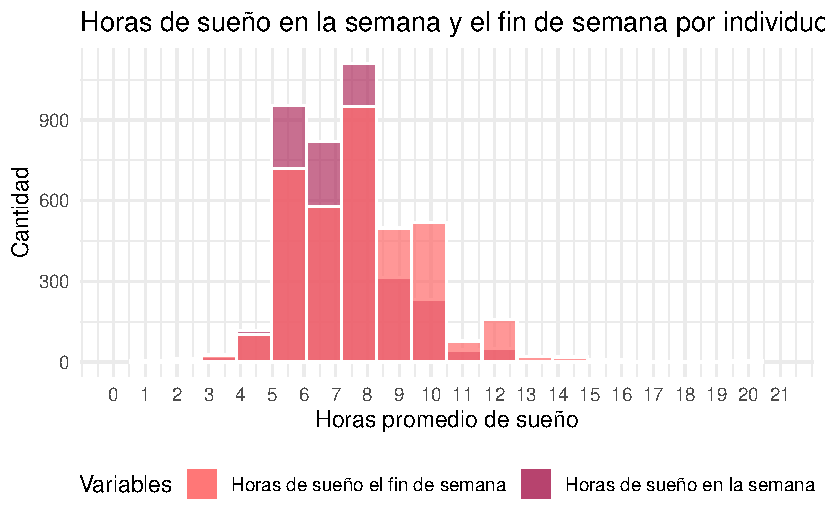
\includegraphics{informe_estadistico_files/figure-pdf/fig-f1-1.pdf}

}

\caption{\label{fig-f1}Comparación de horas de sueño días de semana v/s
fin de semana}

\end{figure}

La figura~\ref{fig-f1} revela que la mayoría de la muestra, tanto
durante la semana como los fines de semana, duerme alrededor de 8 horas.
Esto sugiere que hay una tendencia generalizada hacia un patrón de sueño
de aproximadamente 8 horas por noche en la muestra estudiada. Sin
embargo, se ve que durante el fin de semana, hay un aumento en el número
de horas de sueño en comparación con los días laborales. Este fenómeno
es común y refleja la práctica extendida de ``compensar'' el sueño
perdido durante la semana laboral mediante un mayor descanso durante los
fines de semana.

\hypertarget{trastorno-del-sueuxf1o-1}{%
\subsubsection{Trastorno del Sueño}\label{trastorno-del-sueuxf1o-1}}

El Trastorno del Sueño se reconoce fácilmente como problemas para dormir
de forma contínua en la noche, para entender si la muestra padece de
este problema, se analizará la presencia o ausencia de algún Trastorno
del Sueño. Este diagnóstico se basa en aquellos individuos que
respondieron afirmativamente a al menos una de las preguntas formuladas
por la Encuesta Nacional de Salud (ENS) en etapas anteriores.

\begin{figure}[H]

{\centering 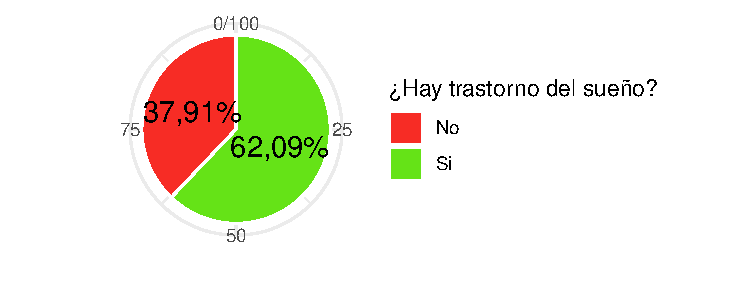
\includegraphics{informe_estadistico_files/figure-pdf/fig-f2-1.pdf}

}

\caption{\label{fig-f2}Presencia de trastorno del sueño en los
individuos de la muestra}

\end{figure}

En la figura~\ref{fig-f2} se ilustra la prevalencia del Trastorno del
sueño dentro de la muestra examinada. Según los resultados,
aproximadamente el 61\% de los participantes de la muestra fueron
identificados como personas que padecen este problema.

\hypertarget{sospecha-de-apnea}{%
\subsubsection{Sospecha de Apnea}\label{sospecha-de-apnea}}

El estudio de la Sospecha de Apnea es útil para evaluar si hay presencia
de apnea en el sueño lo cuál tiene un impacto directo en los resultados
obtenidos anteriormente. Al examinar la relación entre la Sospecha de
apnea y el Estado nutricional, se podría identificar posibles
asociaciones o correlaciones entre estas variables. Esto podría ayudar a
comprender mejor cómo factores como el peso corporal o el Índice de Masa
Corporal (IMC) pueden estar relacionados con la presencia de apnea del
sueño y, a su vez, cómo estas condiciones pueden influir en otros
aspectos de la salud y los resultados obtenidos en el estudio.

\begin{figure}[H]

{\centering 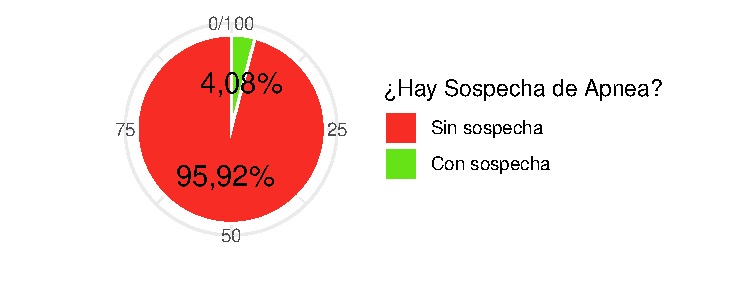
\includegraphics{informe_estadistico_files/figure-pdf/fig-f3-1.pdf}

}

\caption{\label{fig-f3}Sospecha de Apnea en los individuos de la
muestra}

\end{figure}

En la figura~\ref{fig-f3}, se destaca que alrededor del 96\% de la
muestra no presenta signos de sospecha de apnea del sueño. Esto podría
explicarse por el hecho de que para ser considerado sospechoso de apnea,
un individuo debía cumplir con múltiples condiciones adicionales. Entre
estas, se encuentra roncar casi todas las noches, experimentar episodios
de interrupción de la respiración durante el sueño y tener dificultades
para mantenerse despierto durante el día.

\hypertarget{estado-nutricional}{%
\subsection{Estado Nutricional}\label{estado-nutricional}}

El Estado Nutricional es otro conjunto de variables de interés para
determinar la posible relación con el trastorno del sueño. Entre estas
variables, destaca principalmente el Estado Nutricional, que clasifica
el estado de salud del individuo según diferentes valores. Algunos de
estos valores se repiten con respecto a los que se presentan, lo que
convierte a esta variable en un buen resumen de la categoría.

\begin{figure}[H]

{\centering 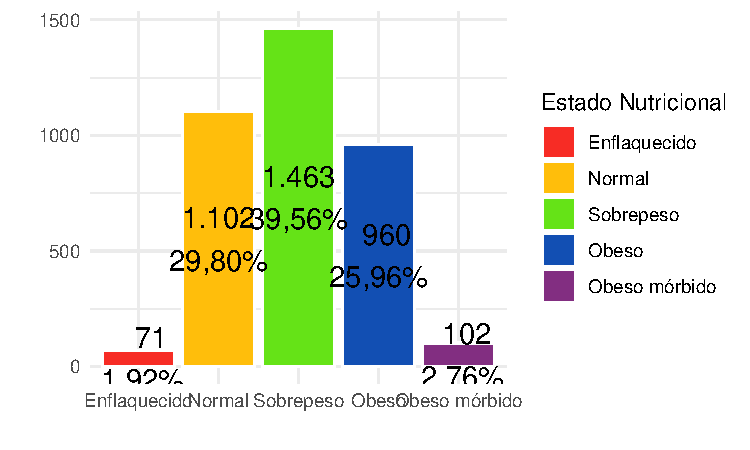
\includegraphics{informe_estadistico_files/figure-pdf/fig-f4-1.pdf}

}

\caption{\label{fig-f4}Estado Nutricional de los individuos de la
muestra}

\end{figure}

De acuerdo a la figura~\ref{fig-f4}, se destaca que la mayoría de los
individuos presentan Sobrepeso, mientras que apenas se registran casos
de ``Enflaquecido'' y ``Obeso mórbido''. Esta información es crucial al
analizar los resultados, ya que ofrece un contexto significativo sobre
la distribución del estado nutricional dentro de la población estudiada.

\hypertarget{metodologuxeda}{%
\subsection{Metodología}\label{metodologuxeda}}

Dado que el objetivo principal de este trabajo es investigar la relación
entre el Trastorno del Sueño y el Estado Nutricional, resulta natural
considerar la correlación entre estas variables para determinar si
existe alguna asociación entre ellas. Esta correlación puede
proporcionar información crucial para entender la naturaleza y la fuerza
de la relación entre ambos aspectos de la salud. Además, explorar
modelos estadísticos puede ayudar a explicar esta relación de manera más
detallada, lo que podría conducir a una comprensión más profunda de los
mecanismos subyacentes y las implicaciones clínicas de dicha asociación.

\begin{figure}[H]

{\centering 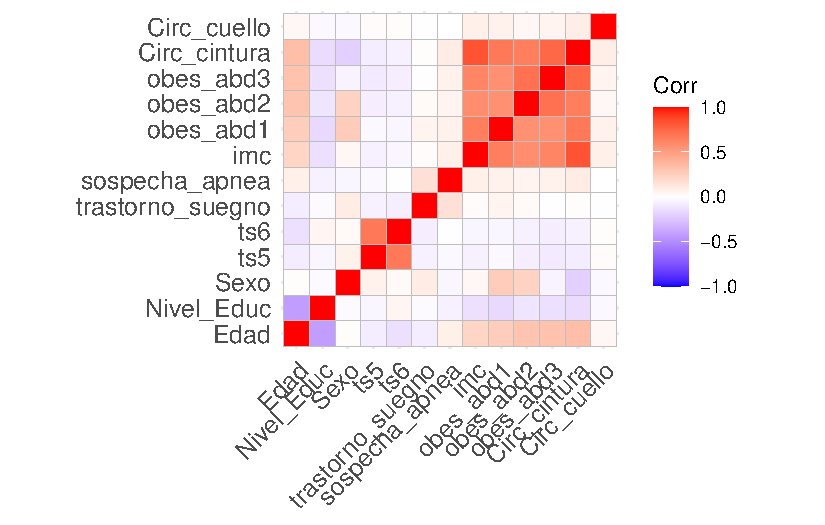
\includegraphics{informe_estadistico_files/figure-pdf/fig-f6-1.pdf}

}

\caption{\label{fig-f6}Correlación}

\end{figure}

En la figura~\ref{fig-f6}, se observa una alta correlación entre las
variables dentro del mismo grupo, ya sea en el grupo del Estado
Nutricional o en el grupo del Trastorno del Sueño. Esto implica que un
modelo lineal no sería la mejor opción para buscar una relación entre
los datos, especialmente considerando que muchas variables en el grupo
del Trastorno del Sueño son dicotómicas.

Dado este escenario, se busca una alternativa para determinar si existe
una relación significativa entre las variables. Varios estudios han
sugerido que los problemas del sueño están relacionados con problemas de
salud, lo que motiva la búsqueda de una prueba estadística que pueda
probar esta hipótesis. Una opción adecuada para este propósito es el
Test Chi-Cuadrado, que permite comparar la relación entre variables
categóricas y determinar si esta relación es significativa. Esta prueba
nos ayudará a evaluar si hay una asociación entre el Trastorno del Sueño
y el Estado Nutricional en nuestra muestra de datos.

\hypertarget{relaciuxf3n-trastorno-del-sueuxf1o-y-estado-nutricional}{%
\subsubsection{Relación Trastorno del Sueño y Estado
Nutricional}\label{relaciuxf3n-trastorno-del-sueuxf1o-y-estado-nutricional}}

Como se ha discutido a lo largo de todo el informe, el objetivo
principal es probar la relación entre estas variables. Para lograr esto,
se empleará el Test Chi-Cuadrado, cuyo propósito es rechazar la
hipótesis nula que afirma que \emph{Las variables son independientes}.
Al revisar la Tabla 5, se presenta:

\begin{table}[H]
  \centering
  \begin{tabular}{lccc}
    \toprule
    Estado Nutricional & Sin trastorno & Con trastorno\\
    \midrule
    Enflaquecido  &   29 &  42 \\
    Normal        &  401 & 701 \\
    Sobrepeso     &  592 & 871 \\
    Obeso         &  345 & 615 \\
    Obeso mórbido &   35 &  67 \\
    \bottomrule
  \end{tabular}
  \caption{Tabla de contingencia de Estado Nutricional v/s Trastorno del Sueño}
  
\end{table}

Aplicando el test Chi-Cuadrado, se obtiene un estadístico Chi-cuadrado
de 7.55 y un valor-p asociado de 0.11. Al considerar una significancia
del 5\%, no se puede rechazar la hipótesis nula, lo que indica que no
podemos concluir que los datos no son independientes. Sin embargo, según
expertos, ``Para aquellos de 50 años a quienes se dio seguimiento a sus
patrones de sueño, las personas que dormían cinco horas o menos por
noche enfrentaban un riesgo 30\% mayor de desarrollar múltiples
enfermedades crónicas con el tiempo que aquellos que dormían al menos
siete horas por noche. A los 60, el riesgo era un 32\% mayor, y a los
70, era un riesgo un 40\% mayor.'' (CNN en Español, 2022). Por lo tanto,
en base a la muestra analizada, no disponemos de suficiente información
estadística para determinar la relación entre estas variables.

\hypertarget{relaciuxf3n-trastorno-del-sueuxf1o-y-edad-de-los-individuos}{%
\subsubsection{Relación Trastorno del Sueño y Edad de los
individuos}\label{relaciuxf3n-trastorno-del-sueuxf1o-y-edad-de-los-individuos}}

Dado que la idea original no pudo ser confirmada, se exploraron
alternativas para determinar si alguna otra variable está relacionada
con los posibles trastornos del sueño. Según la literatura, se sabe que
``los trastornos del sueño son muy frecuentes en los ancianos''
(Gómez-García, 2007). Por lo tanto, al analizar la Tabla 6, se realizó
un cruce de datos entre ambas variables.

\begin{table}[H]
  \centering
  \begin{tabular}{lccc}
    \toprule
    Edad & Sin trastorno & Con trastorno\\
    \midrule
    15 a 24 años  & 218 & 451 \\
    25 a 44 años  & 492 & 874 \\
    45 a 64 años  & 526 & 807 \\
    65 años o más & 297 & 397 \\
    \bottomrule
  \end{tabular}
  \caption{Tabla de contingencia de Edad v/s Trastorno del Sueño}
  
\end{table}

Aplicando el test Chi-Cuadrado resulta el estadístico Chi-cuadrado como
18.51 y un valor-p asociado de 0, con una significancia del 5\%, se
rechaza la hipótesis nula, lo que indica que los datos no son
independientes y sugiere una relación entre el trastorno del sueño y la
variable de edad. A pesar de no encontrar una relación entre los datos
del trastorno del sueño y el estado nutricional, sí es posible
determinar que existe una tendencia con la edad.

\hypertarget{conclusiones}{%
\subsection{Conclusiones}\label{conclusiones}}

Se puede concluir que, a pesar de la amplia evidencia que sugiere una
relación entre el estado nutricional y los trastornos del sueño, los
análisis estadísticos realizados no han logrado corroborar esta
asociación en la muestra estudiada. Aunque se esperaba encontrar una
conexión significativa entre ambas variables, los resultados obtenidos
indican que no hay suficiente evidencia para afirmar una relación
directa entre el estado nutricional y los trastornos del sueño en la
población analizada.

Este hallazgo resalta la complejidad de los factores que pueden influir
en los trastornos del sueño y la necesidad de considerar múltiples
variables para comprender mejor esta relación. Se sugiere que futuras
investigaciones exploren otros factores que podrían estar involucrados,
como los hábitos alimenticios, la actividad física y el estilo de vida
en general. Estos aspectos podrían ofrecer una visión más completa de
los determinantes de los trastornos del sueño y su relación con el
estado nutricional.

Además, se destaca la importancia de llevar a cabo estudios
experimentales más detallados que permitan controlar variables
adicionales y establecer relaciones causales entre el estado nutricional
y los trastornos del sueño. Esto podría proporcionar una comprensión más
sólida de la influencia que el estado nutricional tiene en la calidad
del sueño y sus implicaciones para la salud pública.

Aunque los resultados actuales no respaldan una asociación directa entre
el estado nutricional y los trastornos del sueño en la muestra
analizada, se plantea la necesidad de investigaciones futuras más
exhaustivas para explorar esta relación en profundidad y comprender
mejor los factores que la influencian.

\newpage
\onecolumn

\hypertarget{bibliografuxeda}{%
\subsection{Bibliografía}\label{bibliografuxeda}}

\begin{enumerate}
\def\labelenumi{\arabic{enumi}.}
\item
  A, S. D., De la C, N. F., Q, S. V., G, G. C., \& N, V. D. (2012).
  RELACIÓN ENTRE ESTADO NUTRICIONAL y SUEÑO EN ESCOLARES DE LA COMUNA DE
  SAN MIGUEL, SANTIAGO, CHILE. Revista Chilena de Nutrición, 39(1),
  30-37.
  https://www.scielo.cl/scielo.php?script=sci\_arttext\&pid=S0717-75182012000100003
\item
  CNN en Español. (2022, 19 de octubre). Dormir menos de cinco horas al
  día aumenta el riesgo de desarrollar múltiples enfermedades crónicas,
  según un estudio. CNN en Español.
  https://cnnespanol.cnn.com/2022/10/19/dormir-sueno-5-horas-riesgo-salud-estudio-trax/
\item
  Gómez-García, T., Ruzafa-Martínez, M., Fuentelsaz-Gallego, C., Madrid,
  J. A., \& Rol, M. Á. (2007). Relación entre la calidad del sueño y la
  calidad de vida en estudiantes universitarios. Psicothema, 19(3),
  389-394.
  https://scielo.isciii.es/scielo.php?script=sci\_arttext\&pid=S1137-66272007000200014
\item
  Martinovic, P. A. A., Barria, A. M. M., Morales, M., Vidal, C. D., \&
  Santana, J. L. (2021). Estado Nutricional, Hábitos alimentarios,
  Actividad física y Horas de Sueño en estudiantes de la Patagonia
  Chilena según las estaciones del año: Estudio Observacional. Revista
  Española de Nutrición Humana y Dietética, 25(2), 237-245.
  https://scielo.isciii.es/scielo.php?script=sci\_abstract\&pid=S2174-51452021000200237
\item
  Prensa Gobierno de Mendoza. (s.f.). ``Dormir no es descansar'': los
  trastornos del sueño y sus consecuencias. Recuperado de
  https://www.mendoza.gov.ar/prensa/trastornos-del-sueno-y-sus-consecuencias-dormir-no-es-descansar/\#:\textasciitilde:text=Se\%20denomina\%20trastornos\%20del\%20sueño,a\%20cabo\%20un\%20buen\%20dormir.
\end{enumerate}



\end{document}
